%!TEX root = Report.tex
\chapter{Measurements And Results}\label{sec:results}

\section{Wedge Experiment}
The plot is shown in Figure \ref{fig:f0}. A linear relation can be seen. For the following measurement of the flow cell we can use the scaling relation \ref{eq:scalrel} an read the value for $\left | \delta_{pix} (1^\circ) \right |$ 
from the plot.

\begin{figure}[H]
\centering
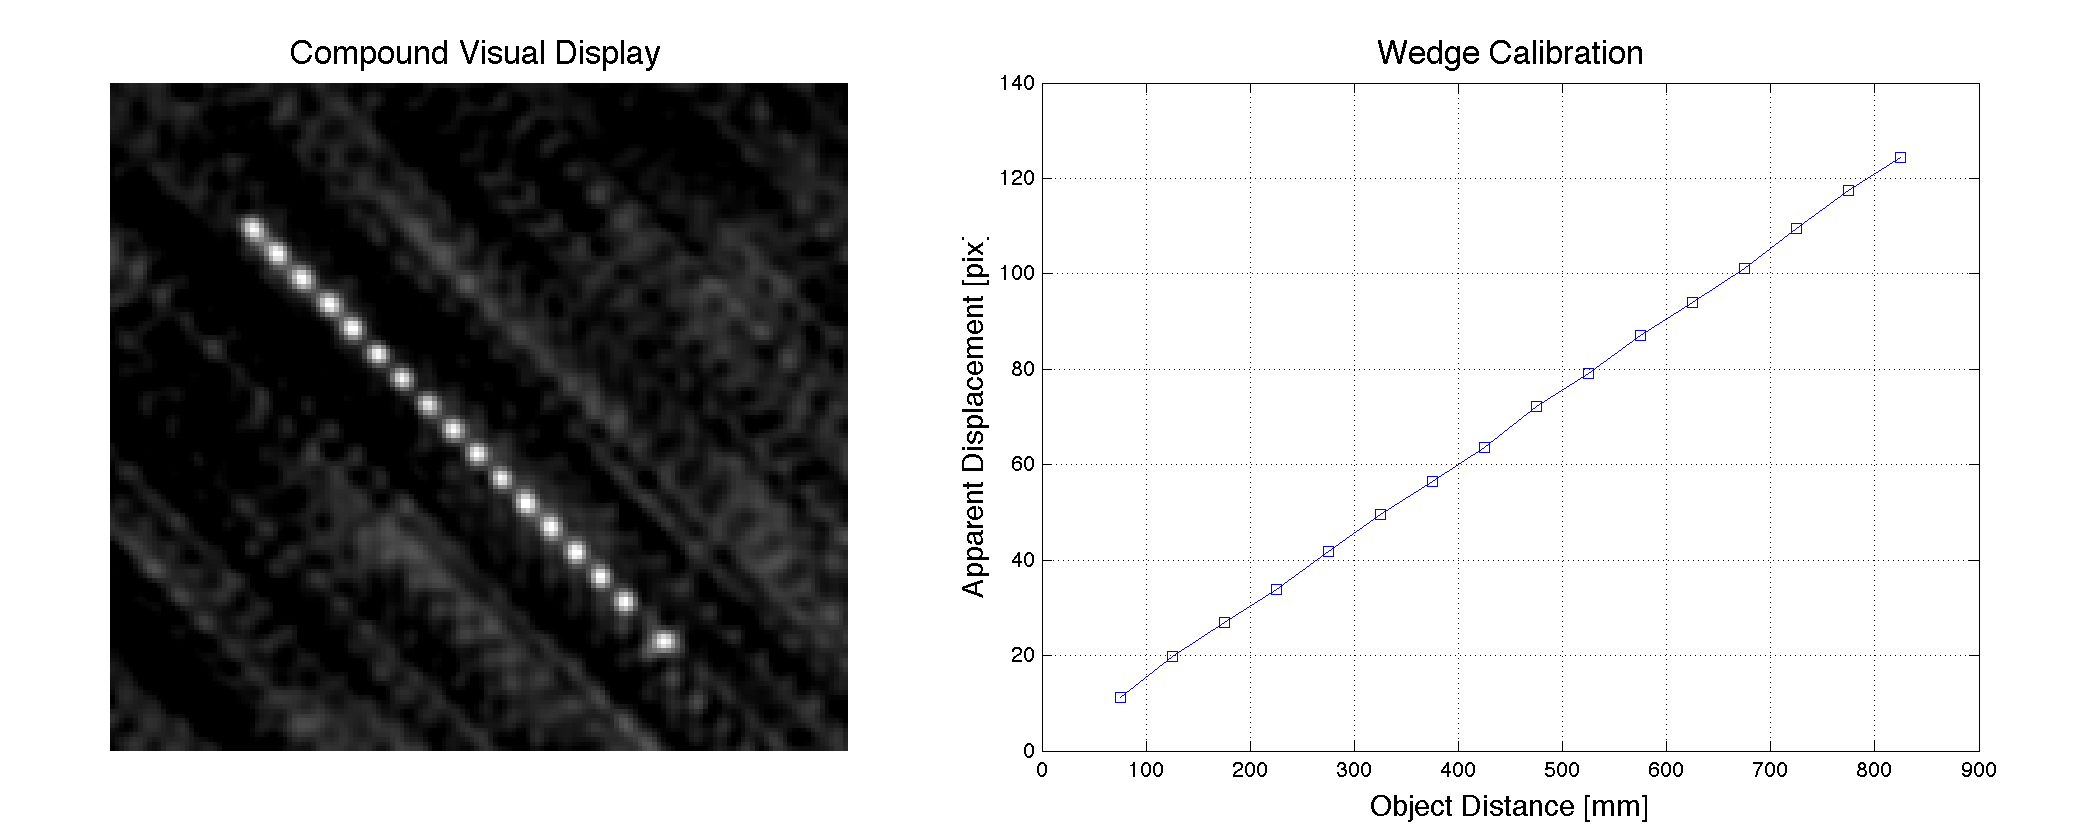
\includegraphics[width=\textwidth]{pics/figure0.png}
\caption{Correlation Peaks And Wedge Calibration}
\label{fig:f0}
\end{figure}



\section{Convection Cell}

After the Wedge Experiment is performed for the calibration of our experimental setup, we proceed to install the probe filled with paraffin. A reference picture was taken before turning on the heating wall on the probe. After turning on the heating system, two pictures were taken at different times whose temperature profile is going to be analysed. The measurements of the probe took place at distance $l = 175 mm $ from the reference background-screen. The reason of chosing one of the first distances on the probe-rail is to reduce the optical deviations.

\begin{figure}[H]
\centering
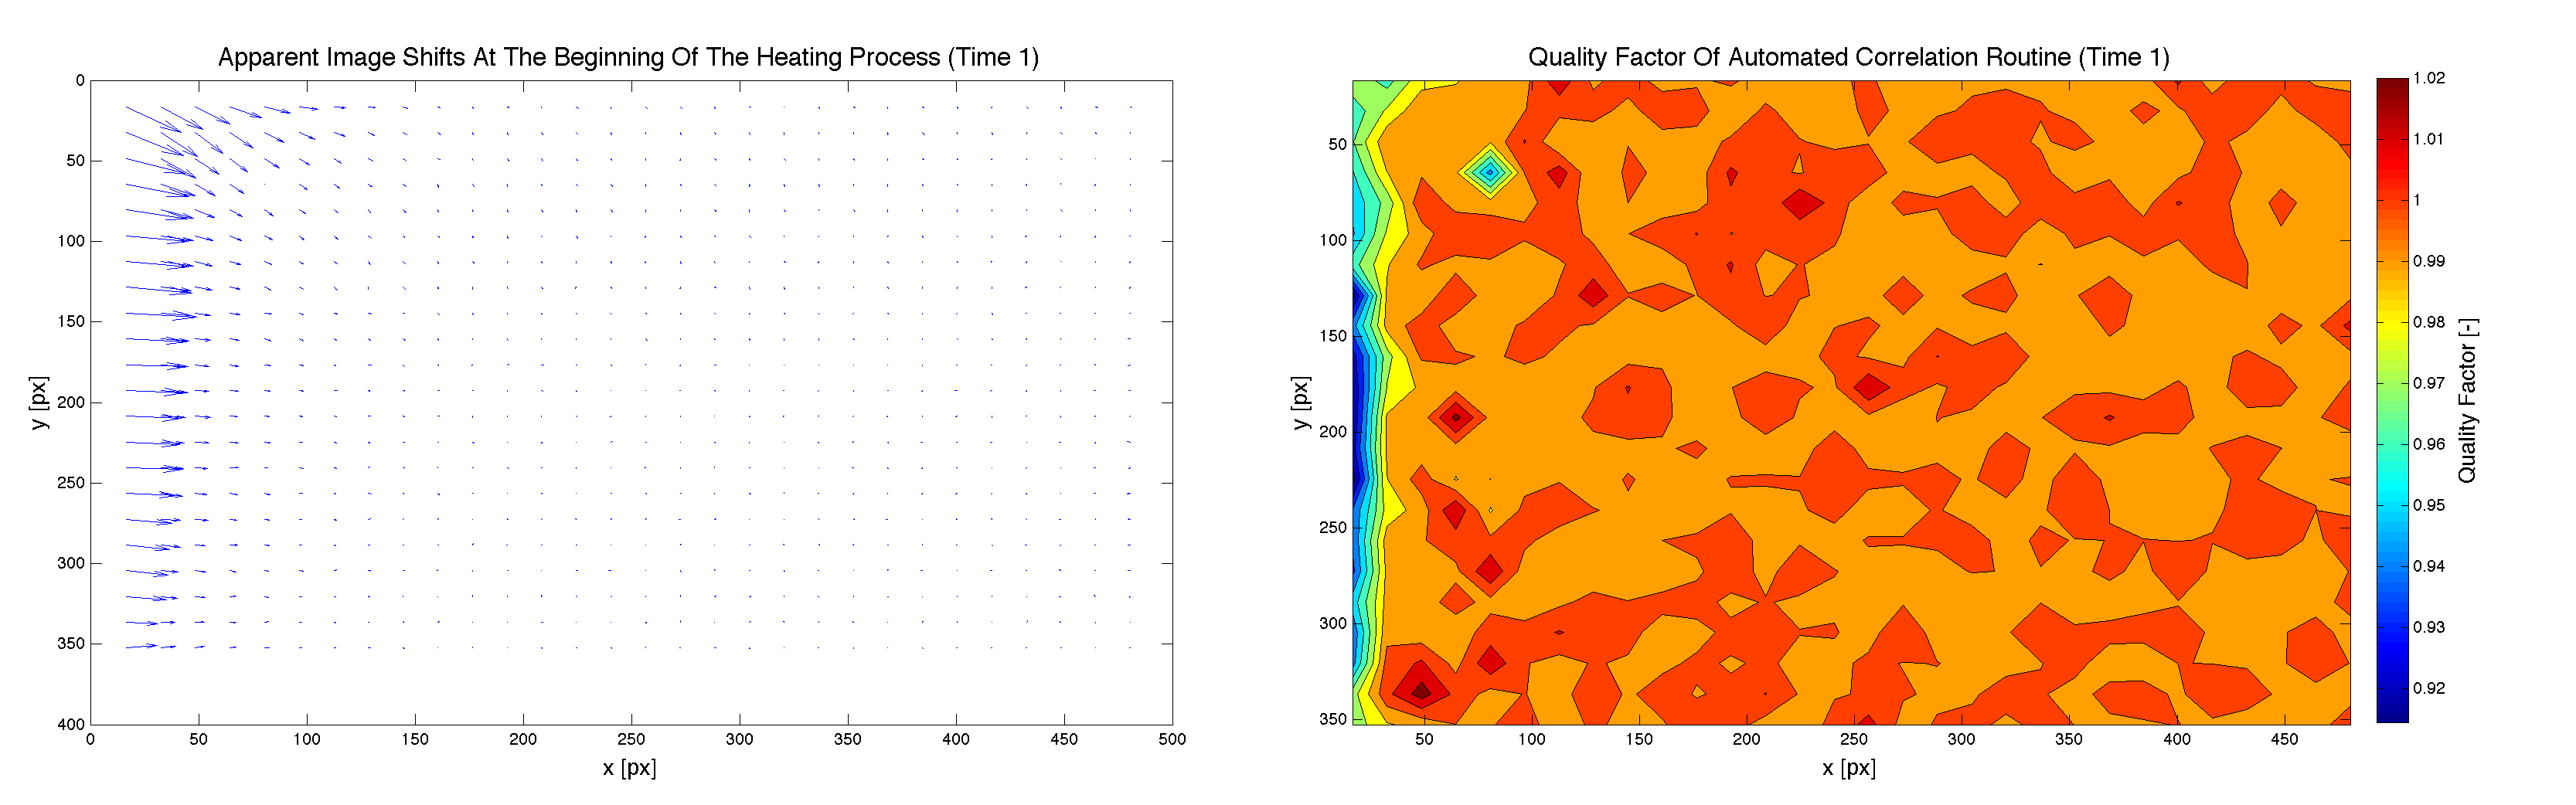
\includegraphics[width=\textwidth]{pics/figure1.png}
\caption{Image Shifts Compared To Reference Image (left) And Calculation Quality Factor (right) At Time 1}
\label{fig:f1}
\end{figure}

On the left side of Figures \ref{fig:f1} and \ref{fig:f2} we observe the field of image deviations of the heated probes compared to the reference unheated probe. We observe in both cases, that the image shifts are more prominent near the heating wall on the left. We also see in the picture taken at a previous time, that the areas further away from the heating source seem practically unaffected (no shift), whereas at the second picture the whole measured field is affected.

\begin{figure}[H]
\centering
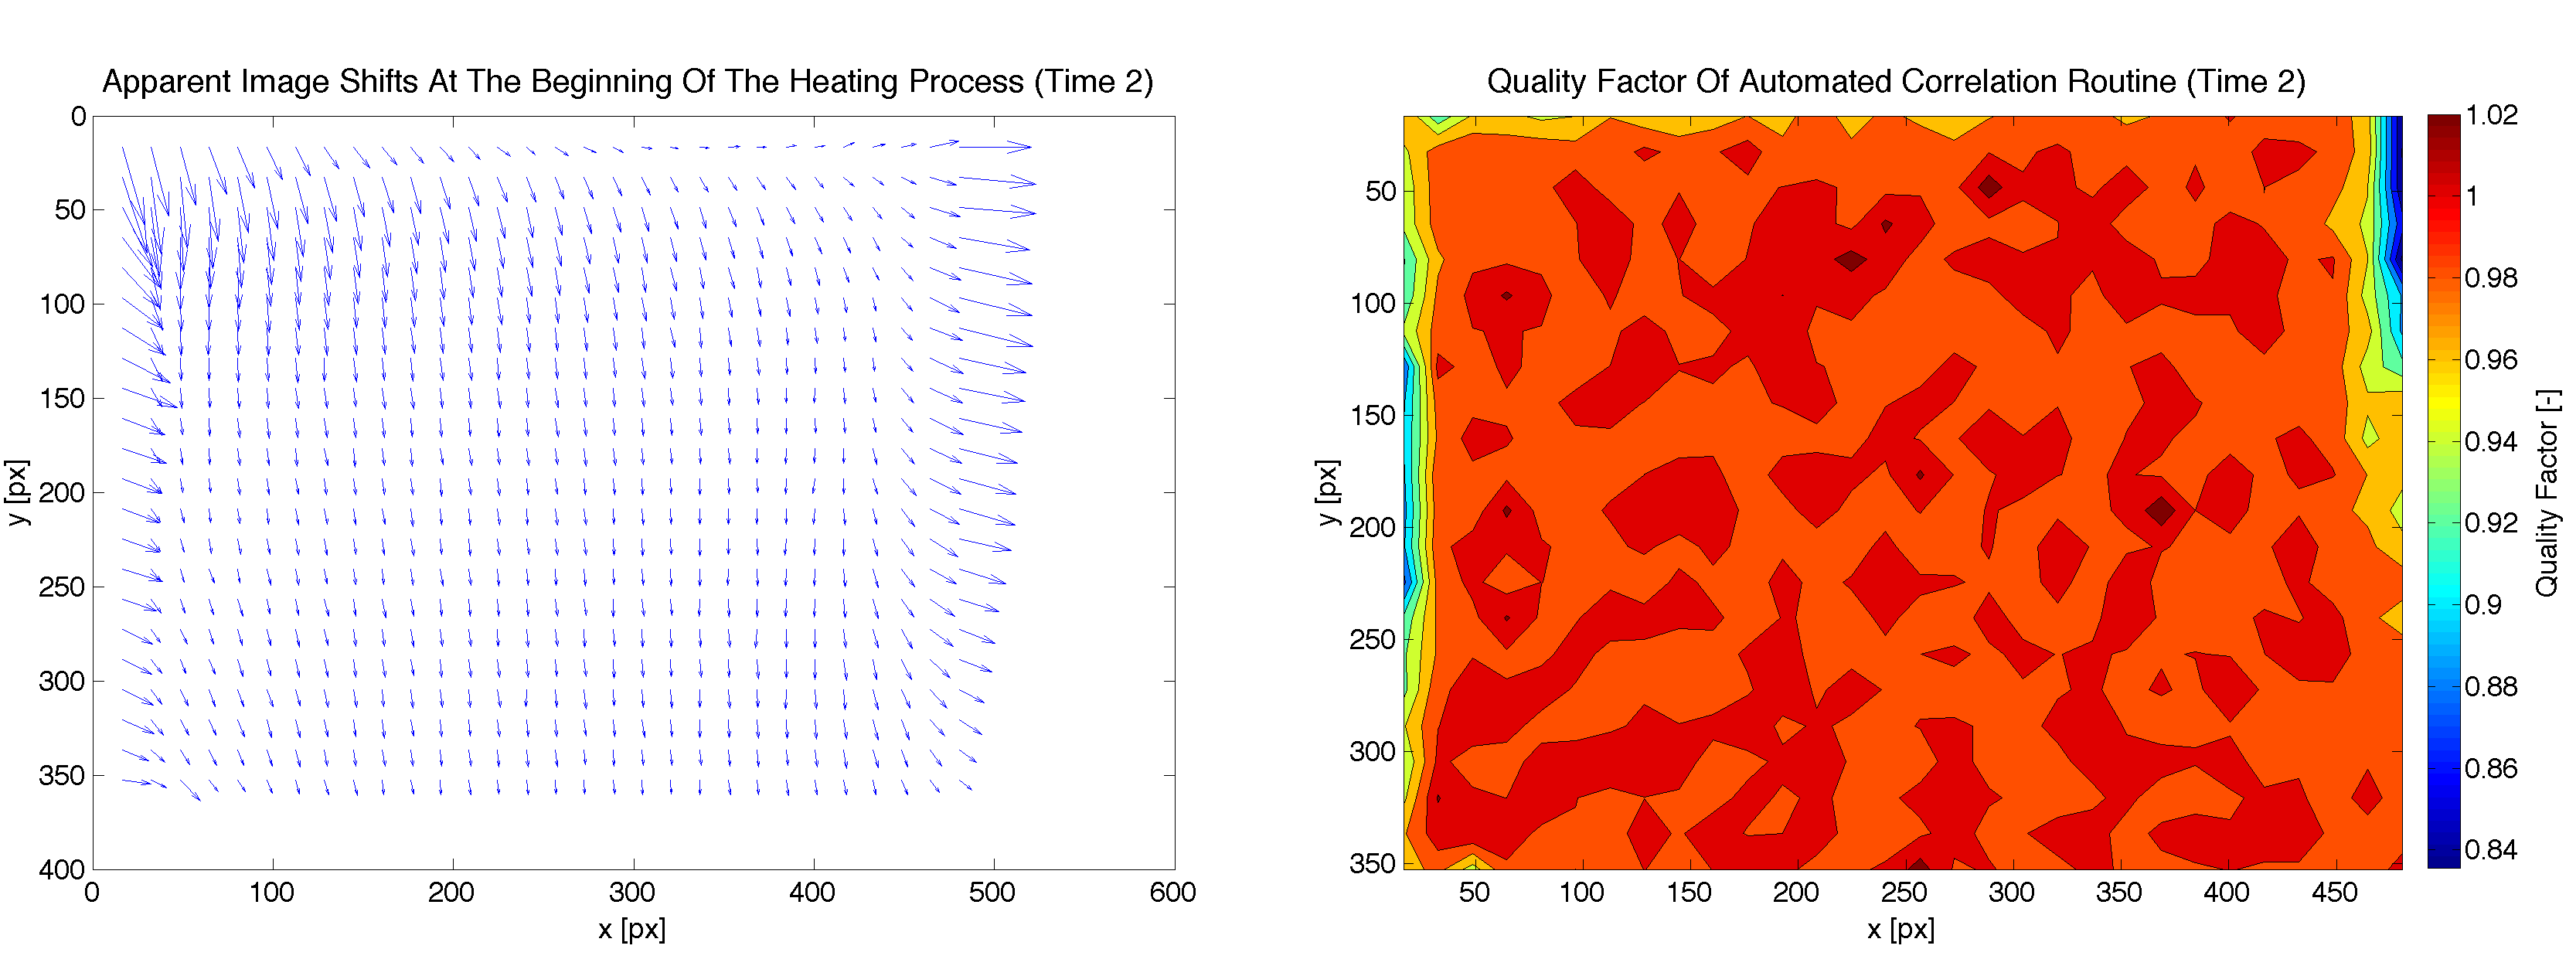
\includegraphics[width=\textwidth]{pics/figure2.png}
\caption{Image Shifts Compared To Reference Image (left) And Calculation Quality Factor (right) At Time 2}
\label{fig:f2}
\end{figure}

In the right part of Figures \ref{fig:f1} and \ref{fig:f2} we observe the quality (or reliability) of the calculation of the mentioned vector field of shifts. The value of the quality is centered around one, which is the best achievable quality. The rectangle in the pictures taken in consideration for the image analysis was chosen according to this quality, so that the shown results are reliable enough (here, between $1.02$ and $0.84$). The reason of the quality being lower on the sides is the irregularity of the image (blurriness) in those areas, as we can see in Figure \ref{fig:refp}.

\begin{figure}[H]
\centering
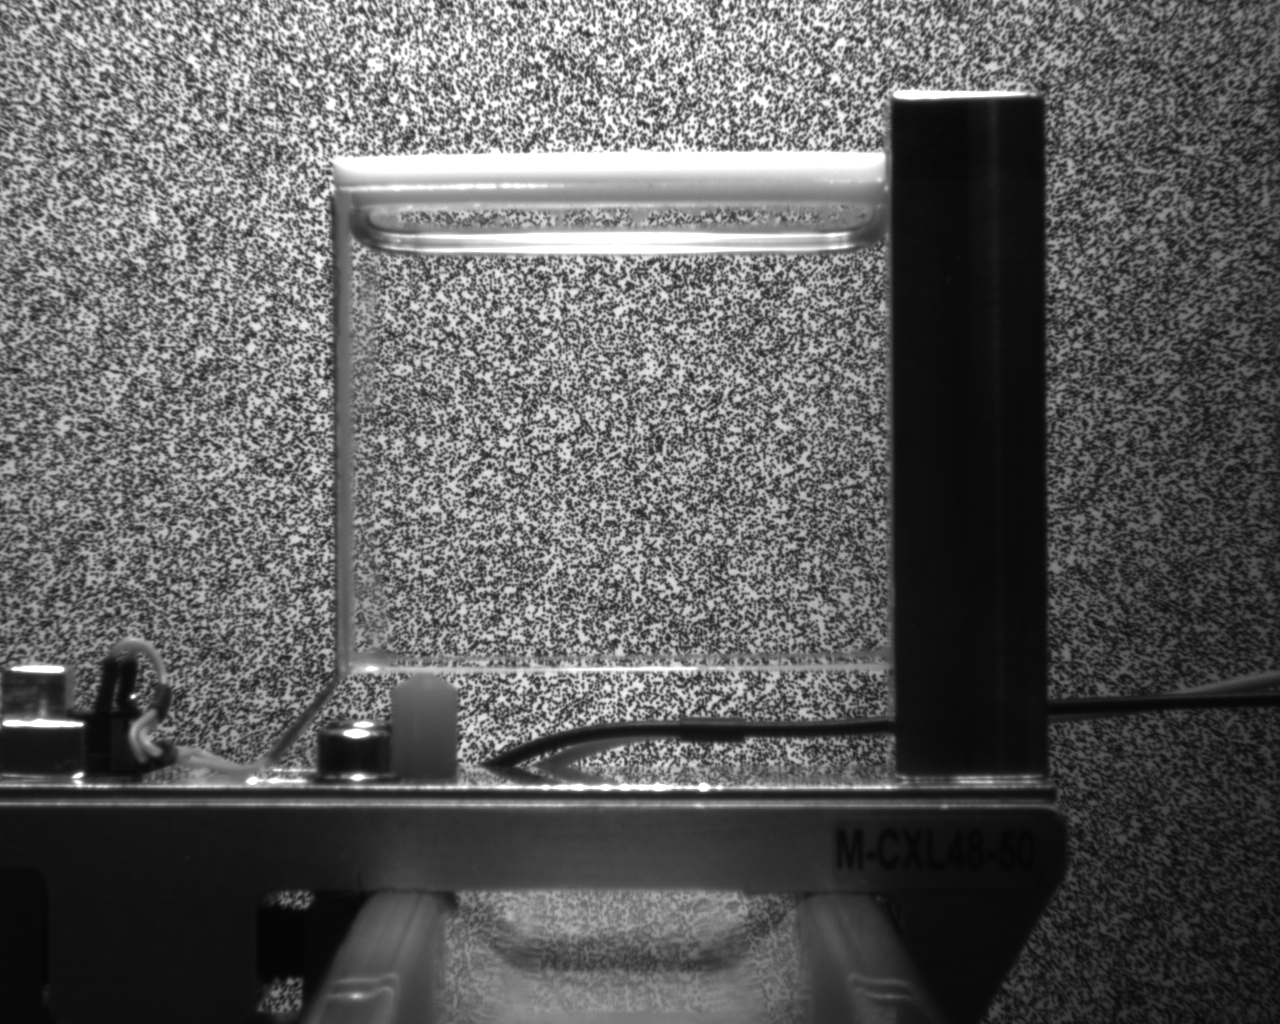
\includegraphics[width=0.5\textwidth]{pics/Referenz_p.png}
\caption{Reference Image at $l=175mm$ (No Heating)}
\label{fig:refp}
\end{figure}

From the relation \ref{eq:gradn} we see clearly that the shift-field shown above is actually proportional to the gradient of $n$. While solving the equation for $n$ and then calculating $T$, or, in other words, calculating the refraction index and the temperature profile out of our image-shifting measurements we get Figure \ref{fig:f3} for Time 1 and Figure \ref{fig:f4} for Time 2. While comparing the corresponding image-shifting-field we see immediately the first mathematical consequence: The shifting vectors are perpendicular to the isopotential lines of $n$ and $T$. 

\begin{figure}[H]
\centering
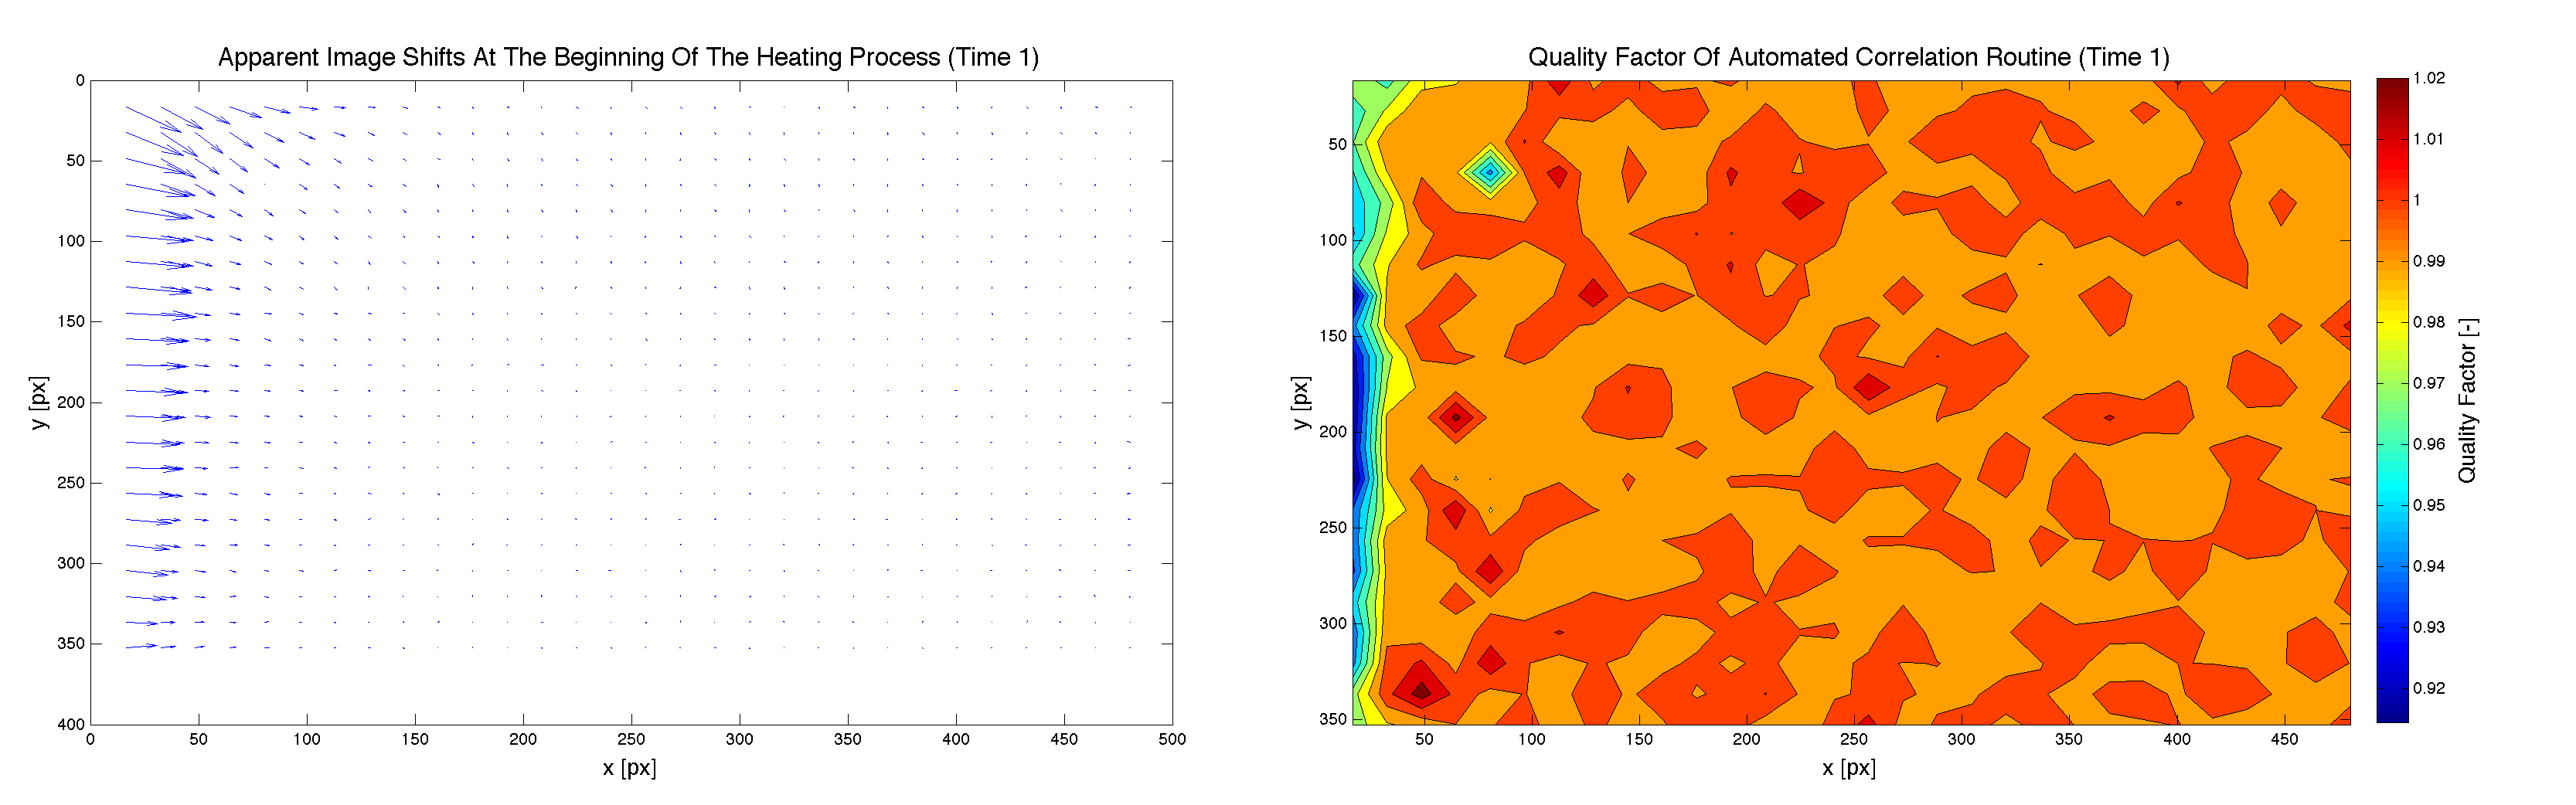
\includegraphics[width=\textwidth]{pics/figure3.png}
\caption{Refraction (Left) And Temperature (Right) Distributions At Time 1}
\label{fig:f3}
\end{figure}

Since the temperature and the defraction index are linearly related, the results look qualitatively similar. We will only discuss the temperature profile, since it's the main objective of this experiments. We observe how the temperature profile shows both thimes a higher temperature near the heating wall. As expected, the distribution of heat is less homogeneous throughout the $x$-axis at later times. Moreover, the paraffin has had more time to get heated and rise it's temperature peak ($24^\circ C$ at Time 1 and $30^\circ C$ at Time 2).\\

The reason that the temperature is highest on the top left an not along the whole heating wall is due to heat convection effects which drive the hotter paraffin to the top. That leads to the uneven heat distbution along the $y$-axis. With this we can understandwhy the gradient field of the image shifts (Figures \ref{fig:f1} and \ref{fig:f2}) is steeper on the upper left part of the probe.

\begin{figure}[H]
\centering
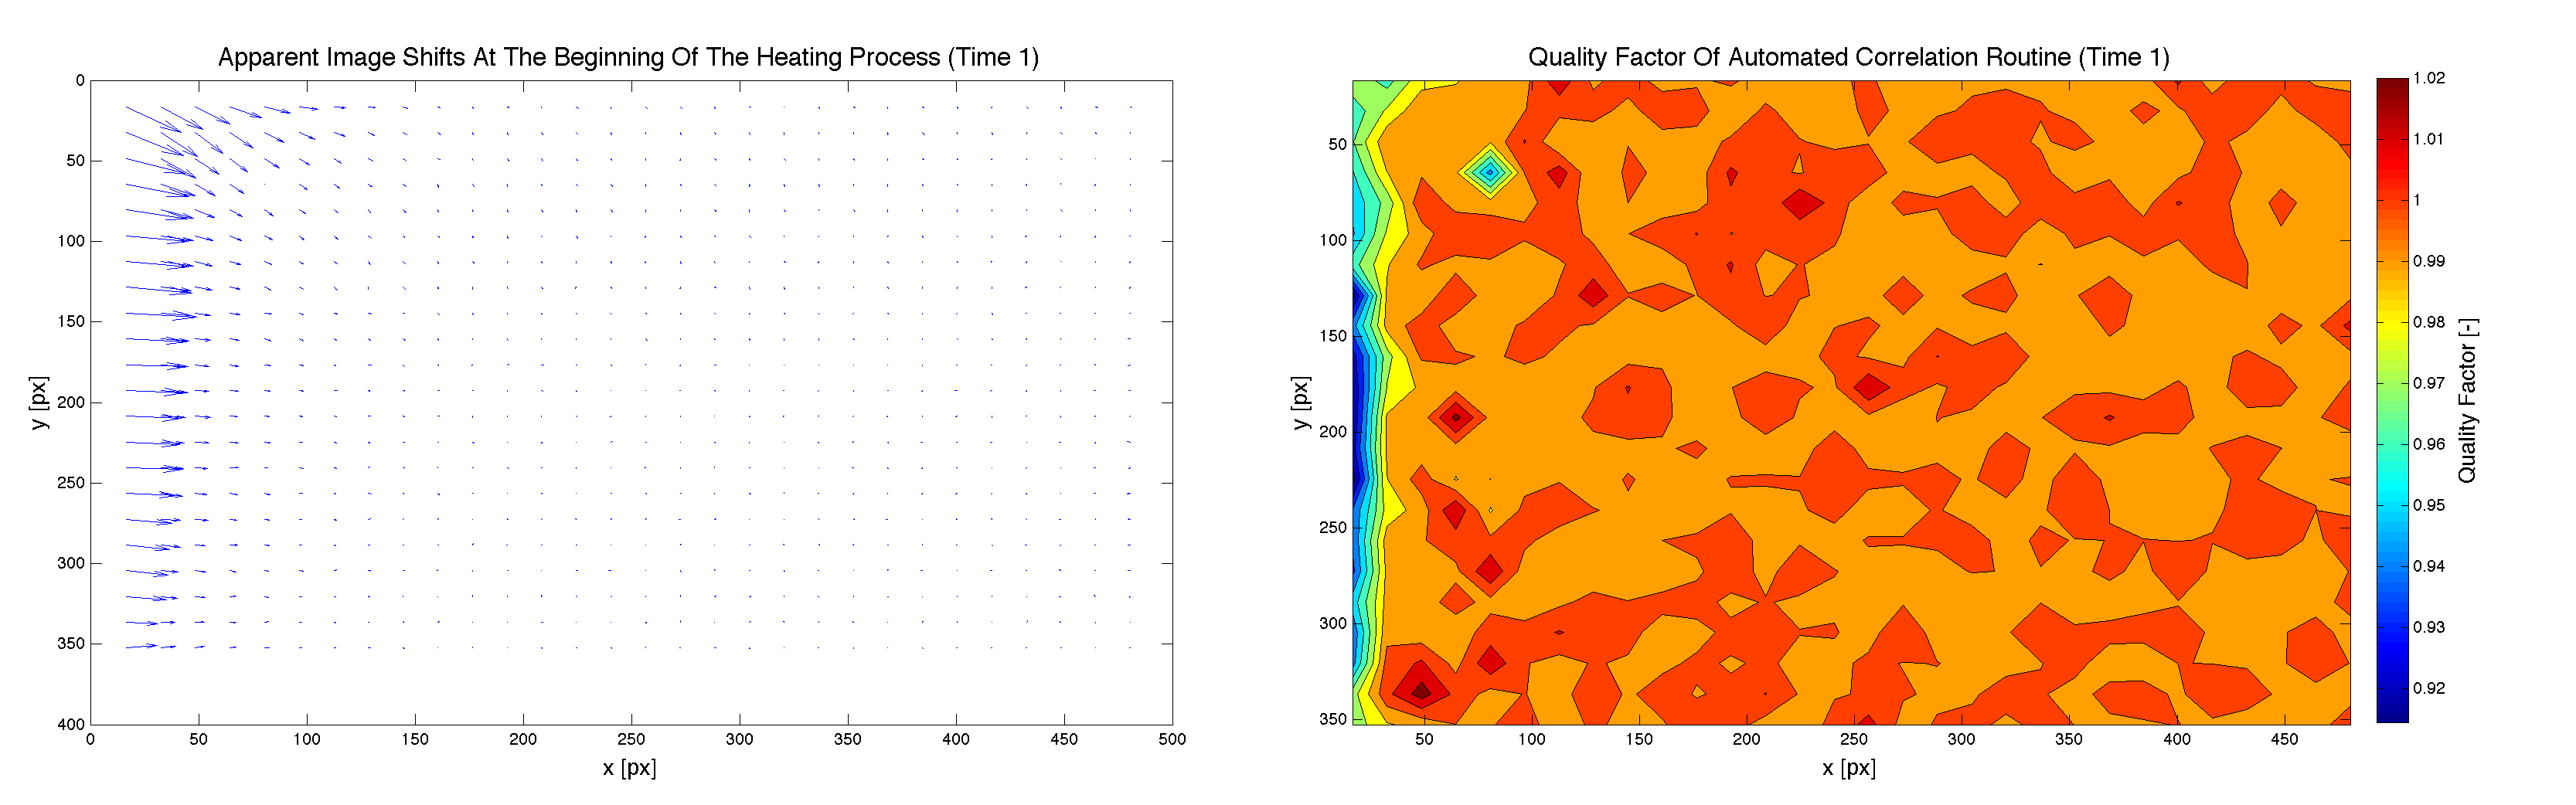
\includegraphics[width=\textwidth]{pics/figure4.png}
\caption{Refraction (Left) And Temperature (Right) Distributions At Time 2}
\label{fig:f4}
\end{figure}